\chapter{La notion de service Web}
\label{section:serviceWeb}

Le projet repose donc sur la cr\'eation d'un service Web.
Son but \'etant de mettre \`a disposition d'un client, des m\'ethodes retournant des informations pour qu'elles soient trait\'ees et affich\'ees.
C'est pourquoi la notion de service Web sera expliqu\'ee dans un premier temps.
Une d\'efinition sera donn\'ee ainsi qu'une architecture basique et le fa\c{c}on dont fonctionne un service Web.
Puis, dans un deuxi\`eme temps, une pr\'esentation de l'API$^*$ utilis\'ee, JAX-WS, pour le d\'eveloppement du service Web sera faite.
Elle permettra de donner un aper\c{c}u des m\'ethodes de d\'eveloppement d'un service Web.

\section{Service Web}

\subsection{D\'efinition}

Un service Web est une application accessible par le r\'eseau, qui permet \`a un client de dialoguer avec le service Web et cela ind\'ependamment de tout langage de programmation et de toute plate-forme d'ex\'ecution.
Un service Web d\'evelopp\'e en Java peut donc \^etre accessible par un client PHP$^*$ par exemple.
C'est un syst\`eme de messagerie standard utilisant le protocole HTTP pour communiquer \`a travers le r\'eseau et s'\'echangeant des fichiers XML.
Son int\'er\^et resulte dans l'utilisation de normes (HTTP et XML) permettant l'int\'erop\'erabilit\'e des services.
De plus, le fait que les services Web n'imposent pas de mod\`ele de programmation sp\'ecifique permet aux vendeurs d'outils de d\'eveloppement d'offrir des m\'ethodes diff\'erentes et donc de facilement diff\'erencier leurs produits de ceux de leurs concurrents.

\subsection{Architecture}

Lorsqu'on parle de services Web, on parle aussi de SOA, \textit{Service-Oriented Architecture} ou architecture orient\'ee services en fran\c{c}ais.
Une architecture orient\'ee services est un style d'architecture qui a pour objectif une interd\'ependance faible entre diff\'erents agents logiciels (module, services).
Les services Web poss\`edent trois normes principales qui sont SOAP, WSDL et UDDI qui permettent respectivement la fa\c{c}on dont les messages sont \'echang\'es, sa description et sa d\'ecouverte.

\subsubsection{\'Echange de messages}

Dans la grande majorit\'e des services Web, le protocole principal de communication est SOAP\protect\footnote{\textit{Simple Object Access Protocol}}.
Il offre le transport d'objets s\'erialis\'es (objets repr\'esent\'es par un flux de bytes) et autres donn\'ees en XML, et l'appel de proc\'edures distantes.

\subsubsection{Description d'un service Web}

Un service Web est d\'ecrit par un document WSDL\protect\footnote{\textit{Web Services Description Language}}.
C'est un langage de description bas\'e sur XML qui permet de donner de fa\c{c}on pr\'ecise les d\'etails concernant le service Web :

\begin{itemize}
	\item son protocole de communication utilis\'e;
	\item le format de messages requis pour communiquer avec le service Web;
	\item les m\'ethodes que le client peut utiliser;
	\item sa localisation.

\end{itemize}

\vspace{0.20cm}

\noindent Un fichier WSDL permet ainsi de savoir comment communiquer avec le service Web.

\subsubsection{D\'ecouverte d'un service Web}

Pour utiliser un service Web, il faut savoir s'il existe.
UDDI\protect\footnote{\textit{Universal Description, Discovery and Integration Service}} est une norme qui d\'efinit le m\'ecanisme pour d\'ecouvrir dynamiquement des services Web.
C'est en fait un annuaire de services permettant de localiser sur le r\'eseau le service Web demand\'e.
\noindent Il comporte :

\begin{itemize}
	\item \textit{des pages blanches}, liste des entreprises ainsi que les informations les concernant;
	\item \textit{des pages jaunes}, liste des services Web de chacunes des entreprises sous le format WSDL
	\item \textit{des pages vertes}, liste des informations techniques pr\'ecises sur les services fournis.

\end{itemize}


\subsection{Fonctionnement}

Le fonctionnement des services Web s'articule autour de trois acteurs principaux illustr\'es par la figure~\ref{figure:schemaServiceWeb}.

\clearpage

\begin{figure}[!ht]
	\centering
	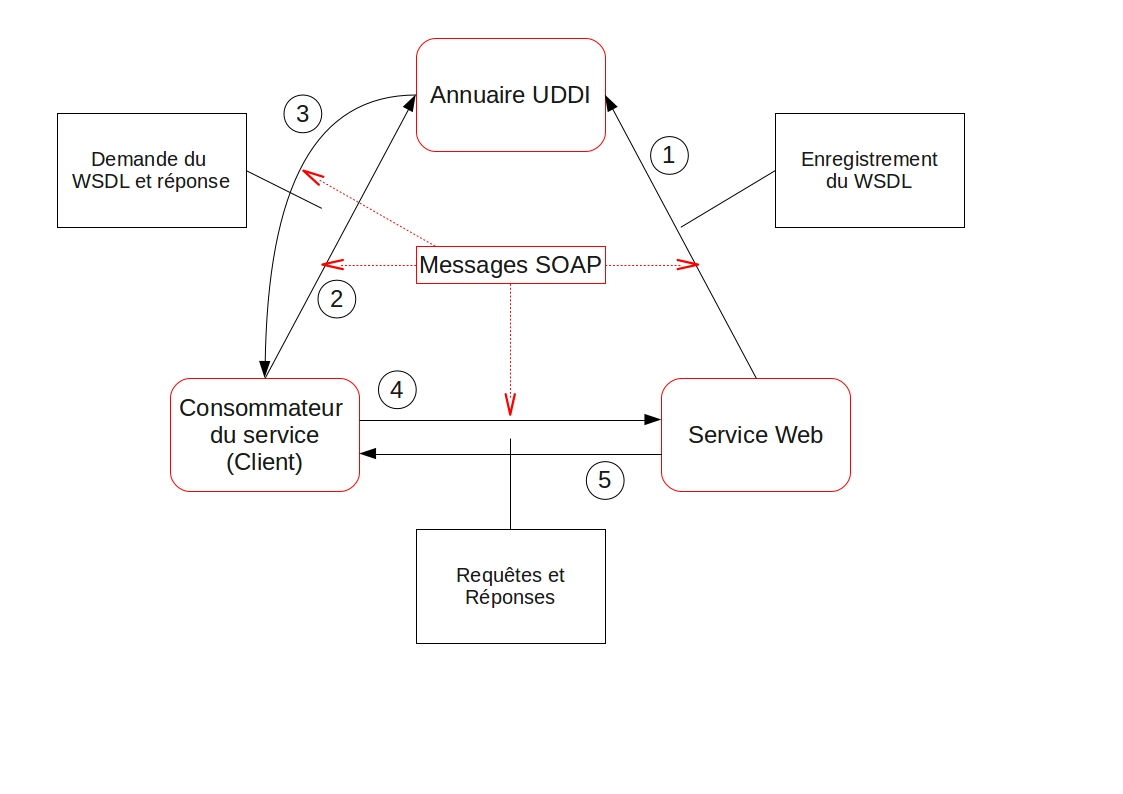
\includegraphics[scale=0.35]{schemaServiceWeb.jpg}
	\caption{Fonctionnement des services Web}
	\label{figure:schemaServiceWeb}

\end{figure}

Les \'etapes impliquant la mise \`a disposition et l'utilisation (consommation) d'un service Web sont les suivantes :

\begin{enumerate}
	\item le service Web d\'ecrit son service en utilisant WSDL. 
	Cette d\'efinition est publi\'ee dans l'annuaire UDDI;
	\item le client envoit une ou plusieurs requ\^ete afin de localiser le service Web \`a l'annuaire et d\'eterminer comment communiquer avec ce service;
	\item une partie du fichier WSDL fourni par le service Web est pass\'e au client. 
	Le client peut maintenant savoir quelles requ\^etes et r\'eponses envoyer au service Web;
	\item le client utilise le fichier WSDL pour envoyer une requ\^ete au service Web;
	\item le service Web fournit la r\'eponse attendue au client.

\end{enumerate}

\section{L'API JAX-WS}

Java API$^*$ for XML Web Services (JAX-WS) est une API Java permettant de simplifier la cr\'eation, le d\'eveloppement et le d\'eploiement de services Web clients et de services Web prestataires.
Il fonctionne avec un syst\`eme d'annotations sp\'ecifique du code Java.
JAX-WS fait partie de la plate-forme Java EE\protect\footnote{\textit{Java Platform, Entreprise Edition}} de Sun Microsystems.
Anciennement appel\'ee JAX-RPC\protect\footnote{\textit{Java API for XML-based RPC}}, ce changement de nom intervient lors de l'abandon du style RPC\protect\footnote{\textit{Remote Procedure Call}}, des appels de proc\'edures distantes, pour des services Web de style document, avec une transmission de donn\'ees au format XML d\'efinies dans un sch\'ema XML.

Toute la partie communication de JAX-WS est g\'er\'ee avec des messages de type SOAP \`a travers HTTP.
L'API$^*$ permet de cacher toute la complexit\'e des messages, le d\'eveloppeur choisit simplement la mani\`ere d'impl\'ementer le service. 
Pour cela, il existe deux m\'ethodes : top-down et bottom-up.

\subsubsection{Top-down}

La m\'ethode top-down permet de d\'evelopper un service Web en partant d'un fichier WSDL.
Ce fichier doit contenir la compl\`ete description de tout le service Web, ensuite le code Java est g\'en\'er\'e automatiquement.
Les classes doivent ensuite \^etre compl\'et\'ees avant d\'eploiement.

\subsubsection{Bottom-up}

La m\'ethode bottom-up permet quant \`a elle de d\'evelopper un service Web en partant du code Java.
Le code Java est d'une part annot\'e, ensuite le fichier WSDL est automatiquement g\'en\'er\'e.
Le service peut enfin \^etre d\'eploy\'e.

\subsubsection{Choix de la m\'ethode et exemple}

C'est la m\'ethode bottom-up qui a \'et\'e employ\'ee dans le projet.
Elle permet de ne se soucier que du code Java, le reste \'etant g\'er\'e automatiquement par NetBeans avec la construction du service Web et le d\'eploiement sur le serveur GlassFish.
NetBeans et GlassFish seront d\'ecrits respectivement aux \S~\ref{section:netbeans} et~\ref{section:glassfish}.
Le code~\ref{code:exempleJAXWS} donne un exemple d'annotations sur un code Java.

\clearpage

\begin{figure}[!ht]
	\lstinputlisting[language=Java]{codes/ExempleService.java}
	%\captionof{figure}{Exemple de classe Java annot\'ee avec JAX-WS}
	\caption{Exemple de classe Java annot\'ee avec JAX-WS}
	\label{code:exempleJAXWS}

\end{figure}

JAX-WS \textit{Reference Implementation} est disponible sur son site Internet\cite{biblio:siteJAXWS} en version 2.2.6.

\clearpage
